\documentclass{report}
\usepackage[utf8]{inputenc}
\usepackage{tikz}
\usetikzlibrary{shapes.geometric, arrows}
\tikzstyle{startstop} = [rectangle, rounded corners, minimum width=3cm, minimum height=1cm,text centered, draw=black, fill=red!30]
\tikzstyle{io} = [trapezium, trapezium left angle=70, trapezium right angle=110, minimum width=3cm, minimum height=1cm, text centered, draw=black, fill=blue!30]
\tikzstyle{process} = [rectangle, minimum width=3cm, minimum height=1cm, text centered, text width=3cm, draw=black, fill=orange!30]
\tikzstyle{decision} = [diamond, minimum width=3cm, minimum height=1cm, text centered, draw=black, fill=green!30]
\tikzstyle{arrow} = [thick,->,>=stealth]

\title{PREDICTION OF GRAPHENE NANOTAPE ELECTRICAL PROPERTIES USING ARTIFICIAL NEURAL NETWORK}
\author{Pablo Rhuam Cavalcante Silva}

% \date{October 2018}

\usepackage{natbib}
\usepackage{graphicx}
\usepackage{subcaption}

\begin{document}

\maketitle

\section{ABSTRACT}
This paper presents an artificial neural network (ANN)-based approach for modelling the correlation between different graphene nanotape configurations and electrical conductivity and transmission valley. The ANN model was trained and validated with laboratory data with multiple graphene nanotape configurations/formats.



\section{INTRODUCTION}
\subsection{DATA SOURCE AND PRE-PROCESSING}

The task is this: predict the conductivity and transmission of a given configuration graphene nanotape.

A bit of information about our dataset features:

\begin{itemize}
    \item \textbf{n\_x} - x-axis number of atoms
    \item \textbf{g\_x} - x-axis number of similar gaussian deformations
    \item \textbf{n\_y} - y-axis number of atoms
    \item \textbf{d1} - x-axis distance between a pair of gaussian deformation
    \item \textbf{b} - 
    \item \textbf{alpha} - gaussian deformations strain parameter 
    \item \textbf{ENERGY} - the amount of electrical energy applied to the graphene nanotape
    \item \textbf{CONDUCTIVITY} - the amount of electrical energy $G(2e^2/h)$
    \item \textbf{TRANSMISSION} - 
\end{itemize}

Down below the data is statistically described:

\begin{figure}
    \centering
    \includegraphics[width=350px]{data_summary.png}
    \caption{Data summary}
    \label{fig:Data Summary}
\end{figure}

Once we will be using artificial neural network on this experiment, we need to make sure the dataset is prepared for such.
Most of the variables values are higher than 1, so we scaled the features in the range [-0.9, 0.9]

Down below the scaled data is statistically described:

\begin{figure}
    \centering
    \includegraphics[width=350px]{scaled_data_summary.png}
    \caption{Scaled data summary}
    \label{fig:Scaled data summary}
\end{figure}

\begin{figure}
    \centering
    \includegraphics[width=350px]{loss_function_per_epoch.png}
    \caption{Loss function per epoch}
    \label{fig:Loss function per epoch}
\end{figure}

\subsection{Validation set}

\section{THEORETICAL MODELING OF ELECTRICAL CONDUCTIVITY PREDICTION}

\section{METHOD}
After identifying various system parameters that influence the output of the graphene nanotape in terms of electrical conductivity, this work employs Artificial Neural Network (ANN) to describe quantitatively, the effects of these parameters on the amount of electrical conductivity. The parameters are logically arranged to elicit desired effects on the targeted outputs. Details of these activities are explained in the following subsections.

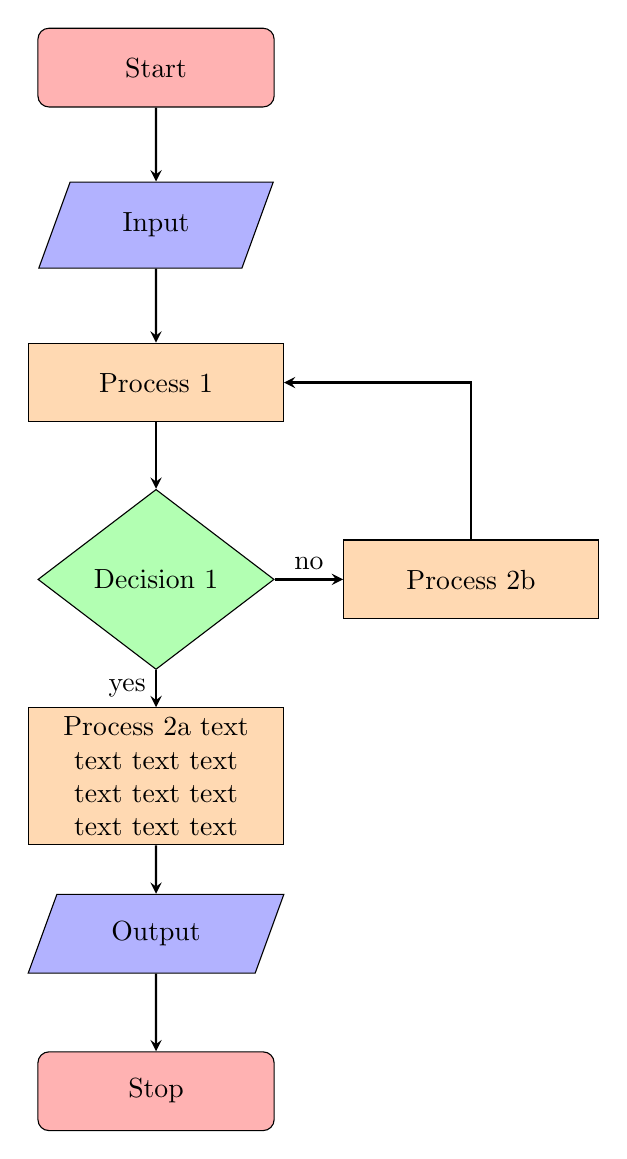
\begin{tikzpicture}[node distance=2cm]

\node (start) [startstop] {Start};
\node (in1) [io, below of=start] {Input};
\node (pro1) [process, below of=in1] {Process 1};
\node (dec1) [decision, below of=pro1, yshift=-0.5cm] {Decision 1};
\node (pro2a) [process, below of=dec1, yshift=-0.5cm] {Process 2a text text text text text text text text text text};
\node (pro2b) [process, right of=dec1, xshift=2cm] {Process 2b};
\node (out1) [io, below of=pro2a] {Output};
\node (stop) [startstop, below of=out1] {Stop};

\draw [arrow] (start) -- (in1);
\draw [arrow] (in1) -- (pro1);
\draw [arrow] (pro1) -- (dec1);
\draw [arrow] (dec1) -- node[anchor=east] {yes} (pro2a);
\draw [arrow] (dec1) -- node[anchor=south] {no} (pro2b);
\draw [arrow] (pro2b) |- (pro1);
\draw [arrow] (pro2a) -- (out1);
\draw [arrow] (out1) -- (stop);

\end{tikzpicture}

\section{RESULTS AND DISCUSSION}

\begin{table}[]
\begin{tabular}{ll}
\textbf{Specification}            &                             \\
Neural Network                    & MLP                         \\
Activation function               & hyperbolic tangent          \\
Learning rate                     & 0.1                         \\
Momentum                          & 0.9                         \\
Number of hidden layers           & 1                           \\
Number of neurons on hidden layer & 10                          \\
Number of neurons on input layer  & 9                           \\
Number of neurons on output layer & 2                           \\
Number of epochs                  & 9                           \\
Solver                            & Stochastic gradient descent
\end{tabular}
\end{table}

\section{CONCLUSIONS}

\bibliographystyle{plain}
\bibliography{references}
\end{document}


